\documentclass{article}
\usepackage{arxiv}

\usepackage[utf8]{inputenc}
\usepackage[english, russian]{babel}
\usepackage[T1]{fontenc}
\usepackage{url}
\usepackage{booktabs}
\usepackage{amsfonts}
\usepackage{nicefrac}
\usepackage{microtype}
\usepackage{lipsum}
\usepackage{graphicx}
\usepackage{natbib}
\usepackage{doi}



\title{Нейронные сети для обнаружения аномалий в многомерных временных рядах}

\author{  Дмитрий Сергеевич Прокудин \\
	Факультет ВМК \\
    МГУ имени М.В.Ломоносова \\
	Москва, Россия \\
	\texttt{TheLoyalist@yandex.ru} \\
	%% examples of more authors
	\And
	Ольга Анатольевна Кравцова \\
	Факультет ВМК \\
    МГУ имени М.В.Ломоносова \\
	Москва, Россия \\
	\texttt{mmp@cs.msu.ru}  \\
	%% \AND
	%% Coauthor \\
	%% Affiliation \\
	%% Address \\
	%% \texttt{email} \\
	%% \And
	%% Coauthor \\
	%% Affiliation \\
	%% Address \\
	%% \texttt{email} \\
	%% \And
	%% Coauthor \\
	%% Affiliation \\
	%% Address \\
	%% \texttt{email} \\
}
\date{}

\renewcommand{\shorttitle}{\textit{arXiv} Template}

%%% Add PDF metadata to help others organize their library
%%% Once the PDF is generated, you can check the metadata with
%%% $ pdfinfo template.pdf
\hypersetup{
pdftitle={A template for the arxiv style},
pdfsubject={q-bio.NC, q-bio.QM},
pdfauthor={David S.~Hippocampus, Elias D.~Striatum},
pdfkeywords={First keyword, Second keyword, More},
}

\begin{document}
\maketitle

\begin{abstract}
    
В данной работе сравниваются модели со сложными архитектурами, предназначенными конкретно для прогнозирования многомерных временных рядов, такие как Autoformer и TimesNet, и модели с более простыми архитектурами, предназначенными для работы с последовательностями в общем, такие как рекуррентные нейронные сети и временные свёрточные нейронные сети. Проводится экспериментальное исследование качества прогноза и обнаружения аномалий данными моделями. Рассматривается два метода обнаружения аномалий: на основе разности предсказанных значений и значений исходного ряда и на основе вероятностного подхода. Эксперименты подтверждают применимость рассмотренных моделей и методов для решения данной задачи и показывают преимущество временных свёрточных сетей над специализированными моделями - при более простой архитектуре точность прогноза оказывается выше. 
\end{abstract}


\keywords{Нейронные сети \and многомерные временные ряды \and обнаружение аномалий}

\section{Введение}
Задача обнаружения аномалий во временных рядах нередко возникает при эксплуатации сложных технологических систем \cite{darban2022deep}, \cite{shalyga2018anomaly}. Их работа описывается множеством величин, изменяющихся во времени. Например, это могут быть показания сенсоров и датчиков или состояния различных устройств во время выполнения процесса \cite{shalyga2018anomaly}. Во время нормальной работы эти значения чаще всего ведут себя регулярным образом с характерными значениями или периодичностью. Аномалией в таких данных является отклонение от типичного поведения. Необходимо уметь выявлять такие участки, так как они могут свидетельствовать о наличии сбоев или неисправностей в системе. Обычно части системы взаимосвязаны, поэтому сбой в одной из них может привести к серии сбоев и в других частях. Более того, даже незначительные отклонения от нормальной работы могут привести к существенным неисправностям через достаточно большой промежуток времени. Такая специфика задачи позволяет использовать нейронные сети для её решения, поскольку они способны обрабатывать большие объёмы данных и определять сложные и долговременные связи между компонентами системы \cite{darban2022deep}, \cite{shalyga2018anomaly}, \cite{kravchik2019efficient}, \cite{nie2023time}.

Изучаются модели глубокого обучения для прогнозирования временных рядов и рассматриваются методы обнаружения аномалий на основе их прогноза. В \cite{darban2022deep}, \cite{wu2022autoformer}, \cite{wu2023timesnet}, \cite{zeng2022transformers} для прогнозирования временных рядов применяются специализированные модели со сложной архитектурой, при этом более простые и обобщённые модели либо не рассматриваются, либо не приводится полноценное сравнение с ними. В данной работе специализированные модели Autoformer \cite{wu2022autoformer} и TimesNet \cite{wu2023timesnet}, показывающие лучшие результаты для прогнозирования временных рядов \cite{wu2023timesnet} на момент написания данной работы, сравниваются c более простыми и обобщёнными рекуррентными LSTM \cite{staudemeyer2019understanding}, GRU \cite{dey2017gatevariants} и свёрточными моделями TCN \cite{bai2018empirical}. Проводится два эксперимента: в первом эксперименте на наборе данных MNIST сравниваются рекуррентные нейронные сети и временные свёрточные сети, и выбирается лучшая архитектура для дальнейшего анализа, во втором эксперименте непосредственно решается задача обнаружения аномалий на примере набора данных SWaT \cite{Goh2016ADT} с применением временных свёрточных сетей TCN \cite{bai2018empirical}, модели Autoformer \cite{wu2022autoformer} и модели TimesNet \cite{wu2023timesnet}.
\section{Постановка задачи}
\label{sec:headings}

Имеется многомерный временной ряд $X = \{x_1, x_2, x_3, ..., x_T\}, x_t \in R^k$, $k$ - количество каналов в ряду. Необходимо реализовать алгоритм $F$, оценивающий аномальность элемента $x_t$ исходного ряда. В данной работе алгоритм состоит из двух независимых частей. Сначала строится алгоритм $N$, позволяющий предсказывать следующие $n$ значений временного ряда по входной последовательности произвольной длины $m$ изначального временного ряда: $N(x_t, ..., x_{t + m} - 1) = y_{1}, ..., y_{n} $. В качестве $N$ рассматриваются нейронные сети, обучение происходит с использованием стандартной функции ошибок MSE: $L = \frac{1}{n} \sum_{i=1}^{n} (x_{t_i} - y_i)^2$. Затем строится алгоритм $C$, определяющий аномальность элемента исходного ряда на основе сравнения его с предсказанным значением алгоритма $N$ для этого же момента времени: $C(x_t, y_t) = a_t$. Формально получаем алгоритм $F(x_t, N, C) = z_t, z_t \in R^m$, где $z_t$ - оценка аномальности элемента $x_t$. В общем случае, размерность $m$ оценки может отличаться от размерности $k$ ряда, например, при оценке аномальности только подвыборки каналов по значениям всех каналов. В данной работе $m$ принимается равным $k$.

\section{Базовый эксперимент}

Все описанные в данной работе эксперименты проводились с применением языка программирования Python и библиотеки PyTorch. 

\subsection{Набор данных MNIST}
В данном эксперименте на наборах данных Sequential MNIST и Permuted MNIST сравнивались рекуррентные сети LSTM и GRU и временная свёрточная сеть TCN. Набор данных Sequential MNIST состоит из изображений рукописных цифр размером $28 \times 28$ пикселей, преобразованных в векторы длины $784$. Набор данных Permuted MNIST представляет собой Sequential MNIST, в котором к каждому вектору применили одну и ту же перестановку. Для каждого набора представлена обучающая (50 тыс. объектов) и тестовая (10 тыс. объектов) выборки.  Для сравнения моделей исследовалось качество классификации последовательностей из этих наборов данных. Дополнительно для модели TCN было проверно качество дорисовки бинаризованных цифр: на вход модели подавалась первая половина бинаризованной последовательности, по которой пошагово прогнозировалась вторая. Затем после преобразования полученной последовательности к изображению размером $28 \times 28$ визуально оценивалось его качество. 

\subsubsection{Обучение и применение моделей}

\begin{itemize}
\item LSTM и GRU.

Моделям на вход подавалась вся последовательность из $784$ элементов, для классификации использовалось последнее скрытое состояние и один линейный слой. Обе модели содержат 1 рекуррентный слой, а размерность внутреннего состояния равна 128. 

\item TCN.

Для задачи классификации модели на вход подавалась вся последовательность из $784$ элементов, использовался последний элемент выходной последовательности и один линейный слой. Для задачи дорисовки на вход подавались первые $783$ элемента последовательности и модель обучалась техникой 'teacher-forcing' предсказывать элементы последовательности с $2$-го по $784$-й. В обеих задачах модель состоит из $8$ TCN блоков, размер внутреннего состояния равен $25$, размер ядра свёртки - $7$.
\end{itemize}

Для обучения LSTM и GRU использовался оптимизатор RMSprop с learning\_rate = $1e-3$, для обучения TCN - Adam с learning\_rate = $2e-3$. LSTM обучалась 50 эпох, GRU обучалась 20 эпох, TCN обучалась 10 эпох для задачи классификации и 50 эпох для задачи дорисовки. Размер батча был равен 64 во всех случаях. 
\subsubsection{Исследование результатов}

Для измерения качества классификации подсчитывалась доля верных ответов на тестовой выборке. Сравнение моделей представлено в таблице.\ref{MNIST}.

\begin{table}[]
\centering
\begin{tabular}{|c|c|c|c|}
\hline
Набор данных & \begin{tabular}[c]{@{}c@{}}LSTM ( $\approx 68$ тыс.\\ параметров)\end{tabular} & \begin{tabular}[c]{@{}c@{}}GRU ( $\approx 52$ тыс.\\ параметров)\end{tabular} & \begin{tabular}[c]{@{}c@{}}TCN ($\approx 66$ тыс.\\ параметров)\end{tabular} \\ \hline
Sequential MNIST & 97.7 & 97.2 & 98.9 \\ \hline
Permuted MNIST & 87.4 & 82.9 & 96.7 \\ \hline
\end{tabular}
\caption{Сравнение качества классификации. Представлены \% верных ответов на тестовой выборке, для каждой модели указано количество обучаемых параметров.}
\label{MNIST}
\end{table}

TCN удалось достичь большей точности на обоих наборах данных при сравнимом количестве параметров. На наборе Permuted MNIST качество LSTM и GRU существенно cнизилось в то время, как у TCN оно осталось приблизительно на том же уровне. Это означает, что TCN гораздо лучше справляется с задачей запоминания долговременных зависимостей между элементами (так как соседние пиксели изображения могут оказаться далеко друг от друга в Permuted MNIST).

Результаты дорисовки цифр представлены на рис.\ref{MNIST_draw}. TCN удалось справиться с данной  задачей - видно, что все дорисованные цифры имеют высокий уровень сходства с оригинальным изображением. 

\begin{figure}[h]
    	\centering
    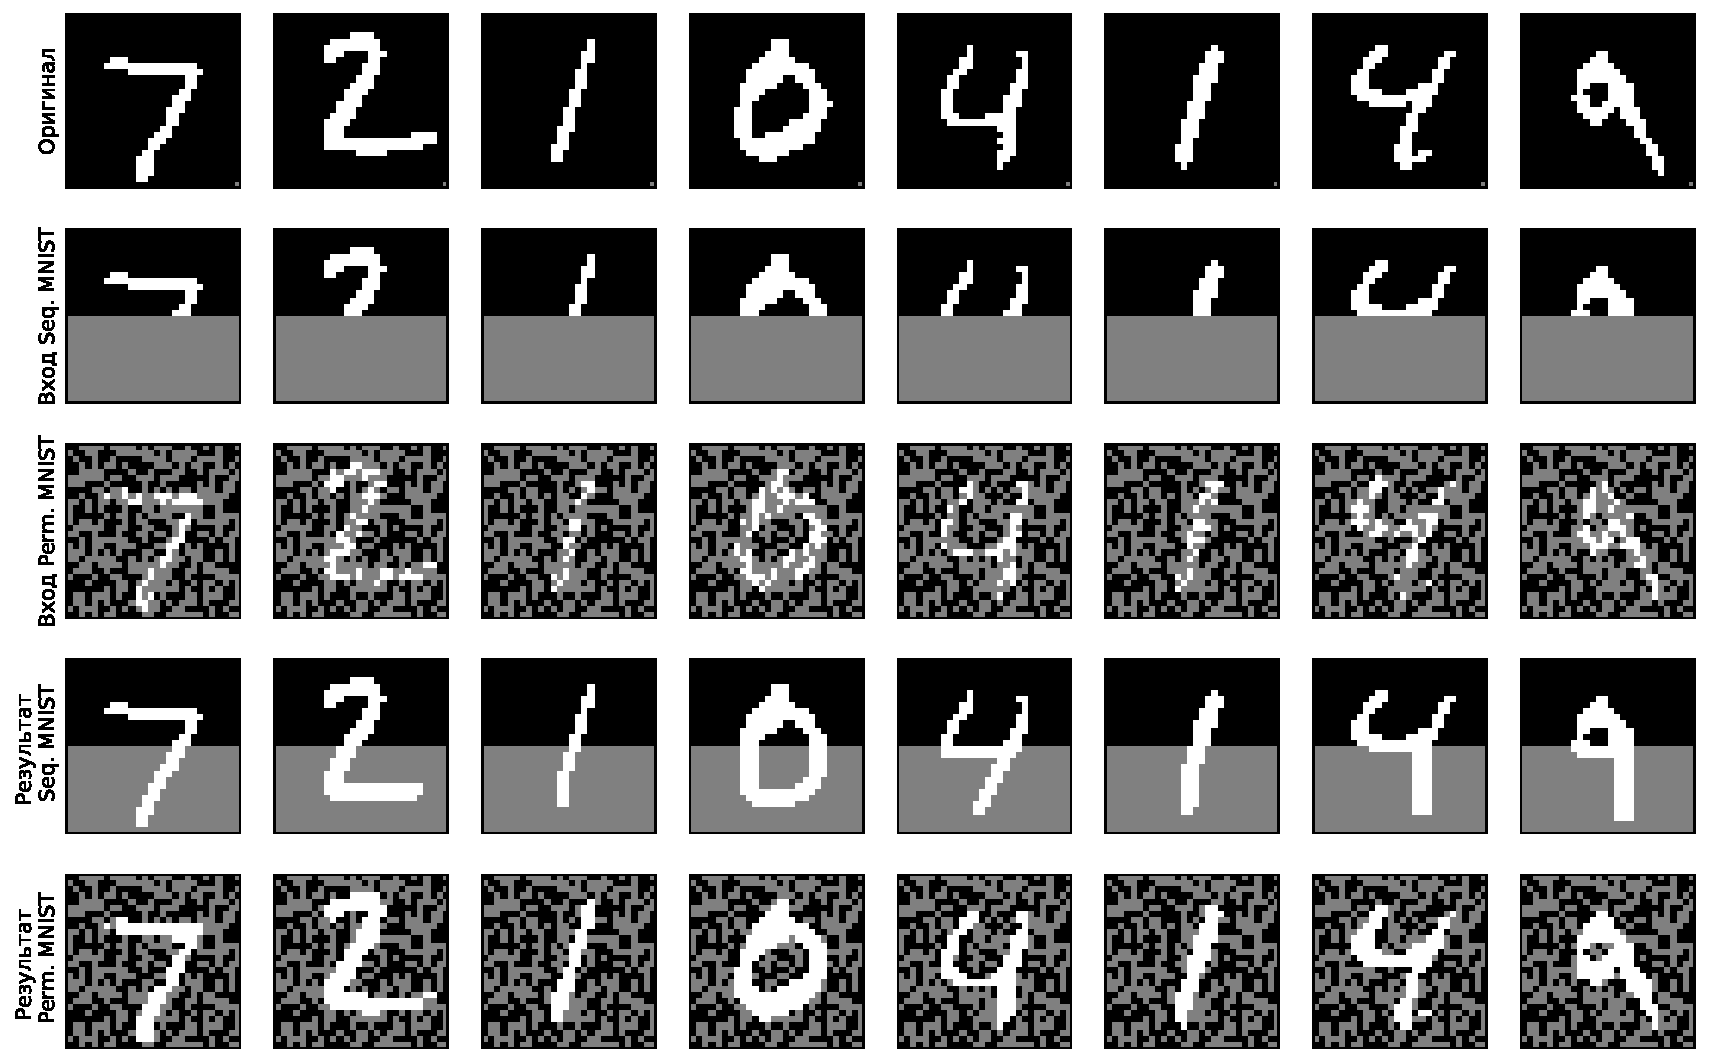
\includegraphics[width=0.8\textwidth]{Kurs_MNIST.pdf}
 	\caption{Результат дорисовки бинаризованных цифр. На входных изображениях серым цветом обозначены элементы, которые не поступали на вход модели.}
 \label{MNIST_draw}
\end{figure}

\subsubsection{Выводы}
\begin{itemize}
\item Эксперимент показал, что TCN лучше запоминает долговременные зависимости между элементами последовательности и качественнее решает задачу классификации цифр.

\item По результатам дорисовки цифр видно, что модель TCN отлично справляется с задачей построения новых элементов последовательности, причём хорошие результаты были достигнуты и для Permuted MNIST, в котором соседние элементы последовательности могут быть никак не связаны друг с другом.

\item На основе полученных выводов было решено, что TCN подходит для задачи прогнозирования временных рядов и обнаружения аномалий лучше, чем рекуррентные нейронные сети. По этой причине в следующем эксперименте рекуррентные сети не исследовались. 
\end{itemize}

\section{Основной эксперимент}

\subsection{Набор данных SWaT}
Иследование качества прогноза и обнаружения аномалий для временного ряда проводилось на наборе данных SWaT \cite{Goh2016ADT}.  Данные описывают технический процесс очистки воды и содержат 51 признак: 26 вещественнозначных замеров с датчиков (например, давление и уровень воды) и 25 дискретных состояний управляющих устройств (например, 'включён-выключен'). Значения записаны с шагом в 1 секунду. Набор разделён на две выборки: 7 неполных дней 'нормальной' работы без аномалий (около 500 тыс. собранных записей) и 6 дней с аномалиями (около 450 тыс. собранных записей). В качестве аномалий выступают атаки на компоненты системы. Всего представлено 36 аномалий: приводится их точная временная разметка, указаны компоненты, на которые была проведена атака, и описание результата атаки. Атаки на систему приводят к нестандартному поведению значений датчиков и состояний управляющих устройств. При этом атака на одну компоненту может повлечь за собой изменения и в других комопнентах, поскольку датчики и устройства системы взаимосвязаны. 

Перед проведением эксперимента данные были агрегированы скользящим медианным окном (размером в 3000 с.) и нормализованы, частота дискретизации была понижена в 10 раз - новые значения признаков соответствуют медианным значениям за последние 10 c. (медианные окна не пересекались).

Из обработанных данных без аномалий были убраны первые 10000 замеров, так как в течение первого дня после запуска система стабилизировалась и поведение значений признаков отличалось от стандартного. Оставшиеся данные были разбиты на подвыборки: обучающую (31500 замеров) и тестовую (8000 замеров) из 'нормальных' данных для обучения и оценки прогноза нейронных сетей, а также валидационную и тестовую выборки из данных с аномалиями для подбора порогов для обнаружения аномалий и оценки качества обнаружения.

Для эксперимента были выбраны следующие 4 признака из 51: 'FIT101', 'LIT101', 'AIT501' (вещественнозначные) и 'MV101' (дискретный). Ряд 'AIT501' был дополнительно приведён к стационарному виду вычитанием среднего значения за последние 500 замеров. Для каждого признака была подготовлена своя разметка аномалий: были выбраны атаки либо на сам признак, либо на коррелирующие с ним признаки. Корреляция выбранных признаков со всеми компонентами системы представлена на рис.\ref{corr_small}.

Пример данных представлен на рис.\ref{example}.

\begin{figure}[H]
    	\centering
    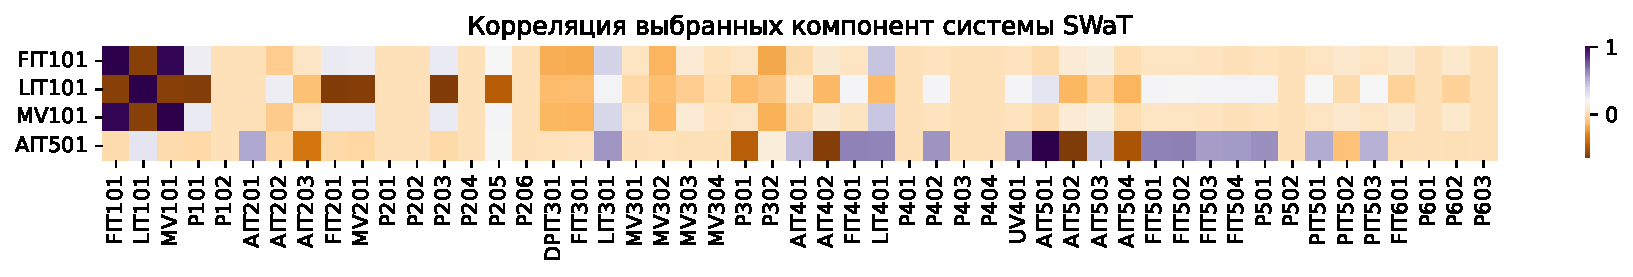
\includegraphics[width=1\textwidth]{corr_small.pdf}
 	\caption{Корреляция выбранных 4 компонент со всеми компонентами системы SWaT. Фиолетовые значения показывают положительную корреляцию, коричневые - отрицательную. Значения датчиков 'FIT101', 'LIT101' сильно коррелируют друг с другом и с состоянием управляющего устройства 'MV101'.}
 \label{corr_small}
\end{figure}

В данном эксперименте сравнивались и исследовались 3 модели: TCN, Autoformer и TimesNet. Для заданного многомерного временного ряда $X = \{x_1, x_2, x_3, ..., x_T\}, x_t \in R^k$ модели обучались по входному сегменту длины $I$ из элементов $x_{t_0}, x_{t_0 + 1}, ..., x_{t_0 + I - 1}$ предсказывать значения для моментов времени $t_1,t_1 + 1, ..., t_1 + L - 1$. Рассматривались два метода обнаружения аномалий:

\begin{enumerate}
\item На основе разности значений прогноза и исходного временного ряда. 

Модели обучались предсказывать значения временного ряда $y_{t_1}, y_{t_1 + 1}, ..., y_{t_1 + L - 1}$. Для обнаружения аномалии в момент времени $t$ проводилась оценка значения разности $y_t$ и $x_t$.

\item На основе вероятностного подхода.

Модели обучались предсказывать параметры нормального распределения значений временного ряда. Для обнаружения аномалии в момент времени $t$ проводится оценка значения стандартного отклонения.
\end{enumerate}

Пороги для оценки и фиксации аномалии подбирались по валидационной выборке. 

Поскольку значения ряда 'MV101' дискретные, то для первого метода всеми моделями прогнозировалась вероятность $\mathcal{P} (MV101 = 1)$, по которой затем определялось значение ряда. Для второго метода ряд 'MV101' не рассматривался. 

\begin{figure}[H]
    	\centering
    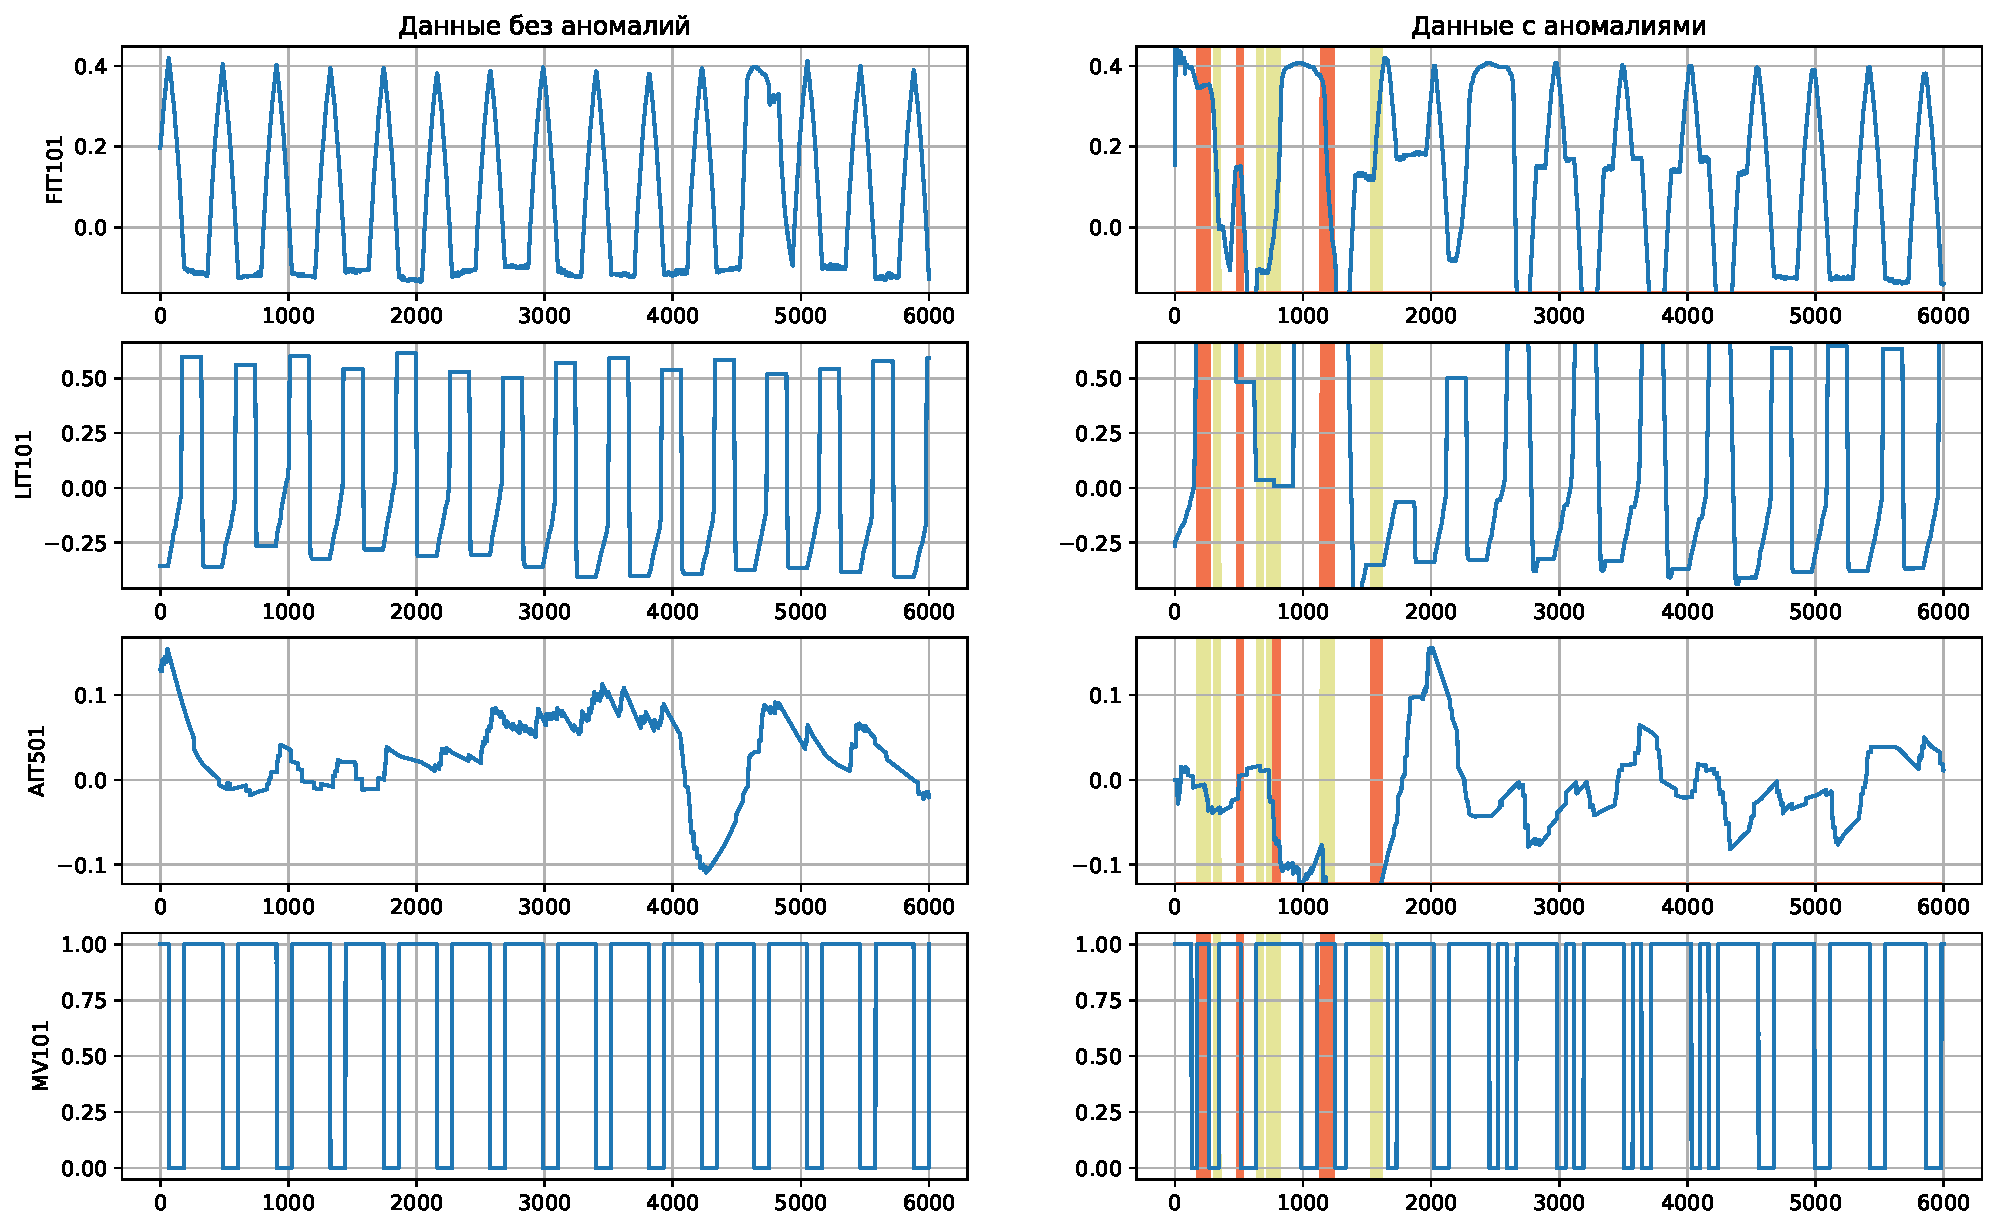
\includegraphics[width=1\textwidth]{examp.pdf}
 	\caption{Пример нормальных данных и данных с аномалиями после предобработки. Признаки 'FIT101', 'LIT101' и 'MV101' имеют сильно выраженную периодичность. Стандартное поведение значений может незначительно варьироваться. На данных с аномалиями изображена разметка аномальных зон: жёлтым цветом отмечены периоды атаки на систему в целом, красным - атаки, связанные с данным признаком. Можно заметить, что не все атаки на систему влияют на каждый признак. В аномальных зонах наблюдаются отличные от нормальных колебания значений, выход значений за стандартные границы и апериодичное поведение.}
 \label{example}
\end{figure}

\subsubsection{Обучение и применение моделей}
Для обучения TCN и TimesNet обучающая выборка была разбита на окна длины $400$ с шагом в $1$ элемент, для Autoformer - на окна длины $100$ с шагом в $1$ элемент. Для первого метода обнаружения аномалий модели обучались предсказывать значения элементов ряда, для второго метода - предсказывать параметры нормального распределния элементов ряда. 

\begin{itemize}
\item TCN.

Модель обучалась техникой 'teacher-forcing' по входной последовательности длины $400$ в моменты времени $t_0, t_0 + 1, ..., t_0 + 399$ предсказывать последовательность длины $400$ из значений для элементов ряда в моменты времени $t_0 + 1, t_0 + 2, ..., t_0 + 400$.

Для построения прогноза тестовая и аномальная выборка были разбиты на окна длины $400$ с шагом в $20$ элементов. Прогноз строится в авторегрессионом формате по 20 элементов.

\item Autoformer.

Модель обучалась по входной последовательности длины $100$ в моменты времени $t_0, t_0 + 1, ..., t_0 + 99$ предсказывать последовательность длины $10$ из значений для элементов ряда в моменты времени $t_0 + 100, t_0 + 101, ..., t_0 + 109$.

Для построения прогноза тестовая и аномальная выборка были разбиты на окна длины $100$ с шагом в $20$ элементов. Модель получала на вход последовательность из элементов ряда и строила прогноз из $10$ элементов, из последовательности убирались первые $10$ элементов, а к концу последовательности добавлялся весь прогноз, затем новая последовательность вновь подавалась на вход модели. Данная процедура повторялась по $2$ раза, после этого в качестве входной последовательности выбиралось следующее окно из выборки.

\item TimesNet.

Модель обучалась по входной последовательности длины $400$ в моменты времени $t_0, t_0 + 1, ..., t_0 + 399$ предсказывать последовательность длины $10$ из значений для элементов ряда в моменты времени $t_0 + 400, t_0 + 401 , ..., t_0 + 409$.

Построение прогноза для TimesNet аналогично построению прогноза для Autoformer, но выборки разбиваются на окна длины $400$. 
\end{itemize}

Для обучения использовался оптимизатор Adam с learning\_rate = $1e-4$, размер батча равнялся $32$ при обучении TimesNet для второго метода и $64$ для всех остальных моделей. Для первого метода обнаружений аномалий все модели обучались $10$ эпох, для второго метода количество эпох варьируется: TCN и TimesNet - $10$, Autoformer - $20$.

\begin{figure}[H]
\centering
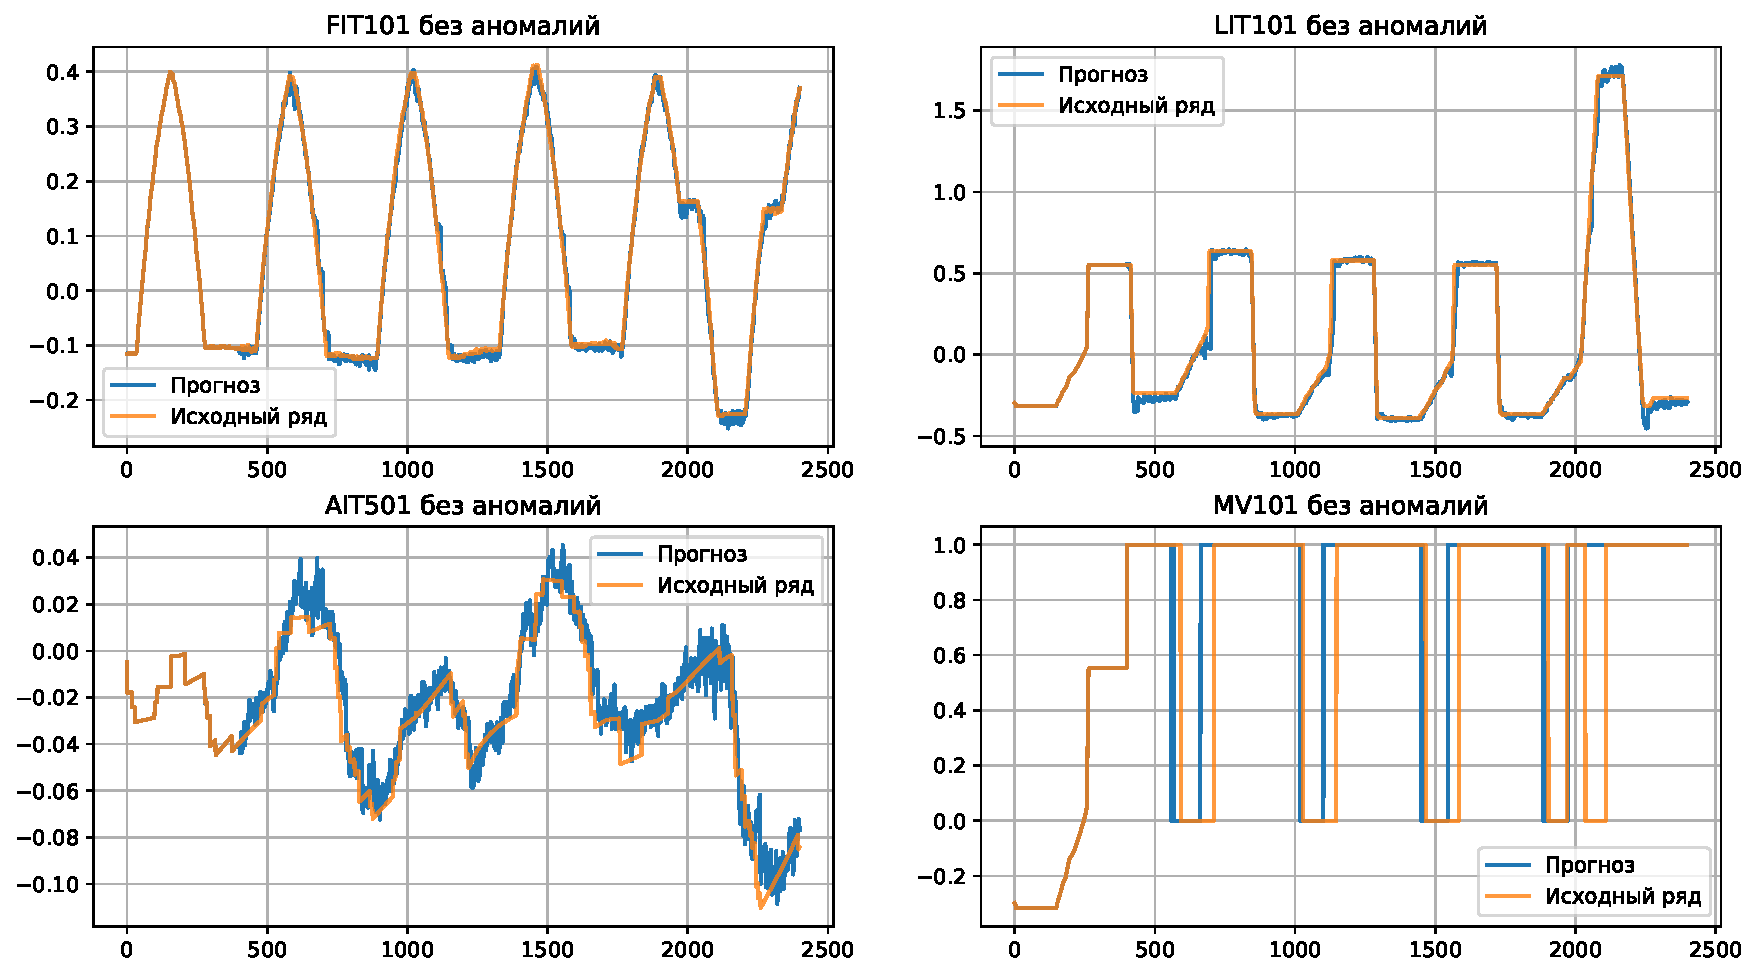
\includegraphics[width=0.9\textwidth]{Test_pred_TCN.pdf}
\caption{Пример прогноза TCN для тестовых данных.}
\label{Test_TCN}
\end{figure}

\begin{figure}[H]
\centering
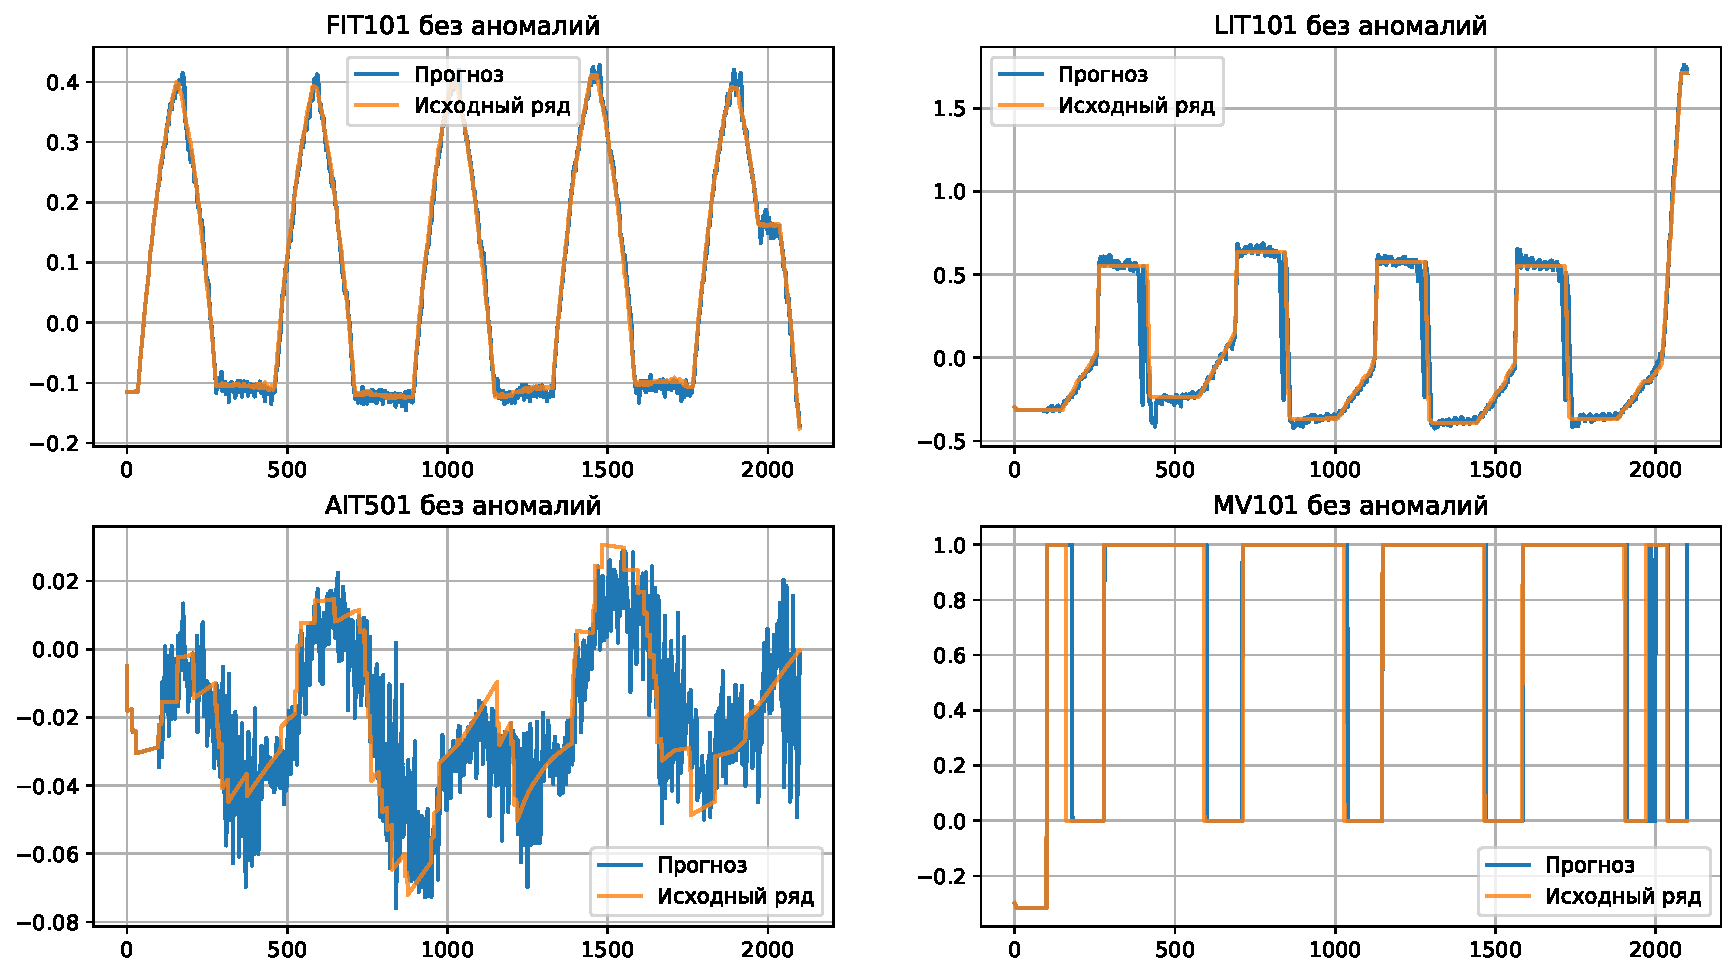
\includegraphics[width=0.9\textwidth]{Test_pred_AF.pdf}
\caption{Пример прогноза Autoformer для тестовых данных.}
\label{Test_AF}
\end{figure}

\subsubsection{Исследование результатов}

Рассмотрим первый метод обнаружения аномалий на основе разности значений и сравним результаты моделей. Прогнозы TCN и Autoformer для тестовой выборки представлены на рис. \ref{Test_TCN}, \ref{Test_AF}, для аномальной - на рис.  \ref{Ano_TCN}, \ref{Ano_AF}. Далее в этом разделе будут показаны графики с анализом только одного ряда 'FIT101'.

Все модели научились точно предсказывать ряды 'FIT101' и 'LIT101' с ярко выраженной периодичностью, достаточно хорошо предсказывались и значения дискретного признака 'MV101'. Хуже всего прогнозировался ряд 'AIT501' с наиболее сложной структурой без выраженной периодичности - прогноз TCN и Autoformer получался 'зашумлённым', а TimesNet не удалось обучить правильно прогнозировать этот ряд. Прогноз модели TCN является наиболее точным и близким к исходному ряду. 

\begin{figure}[H]
\centering
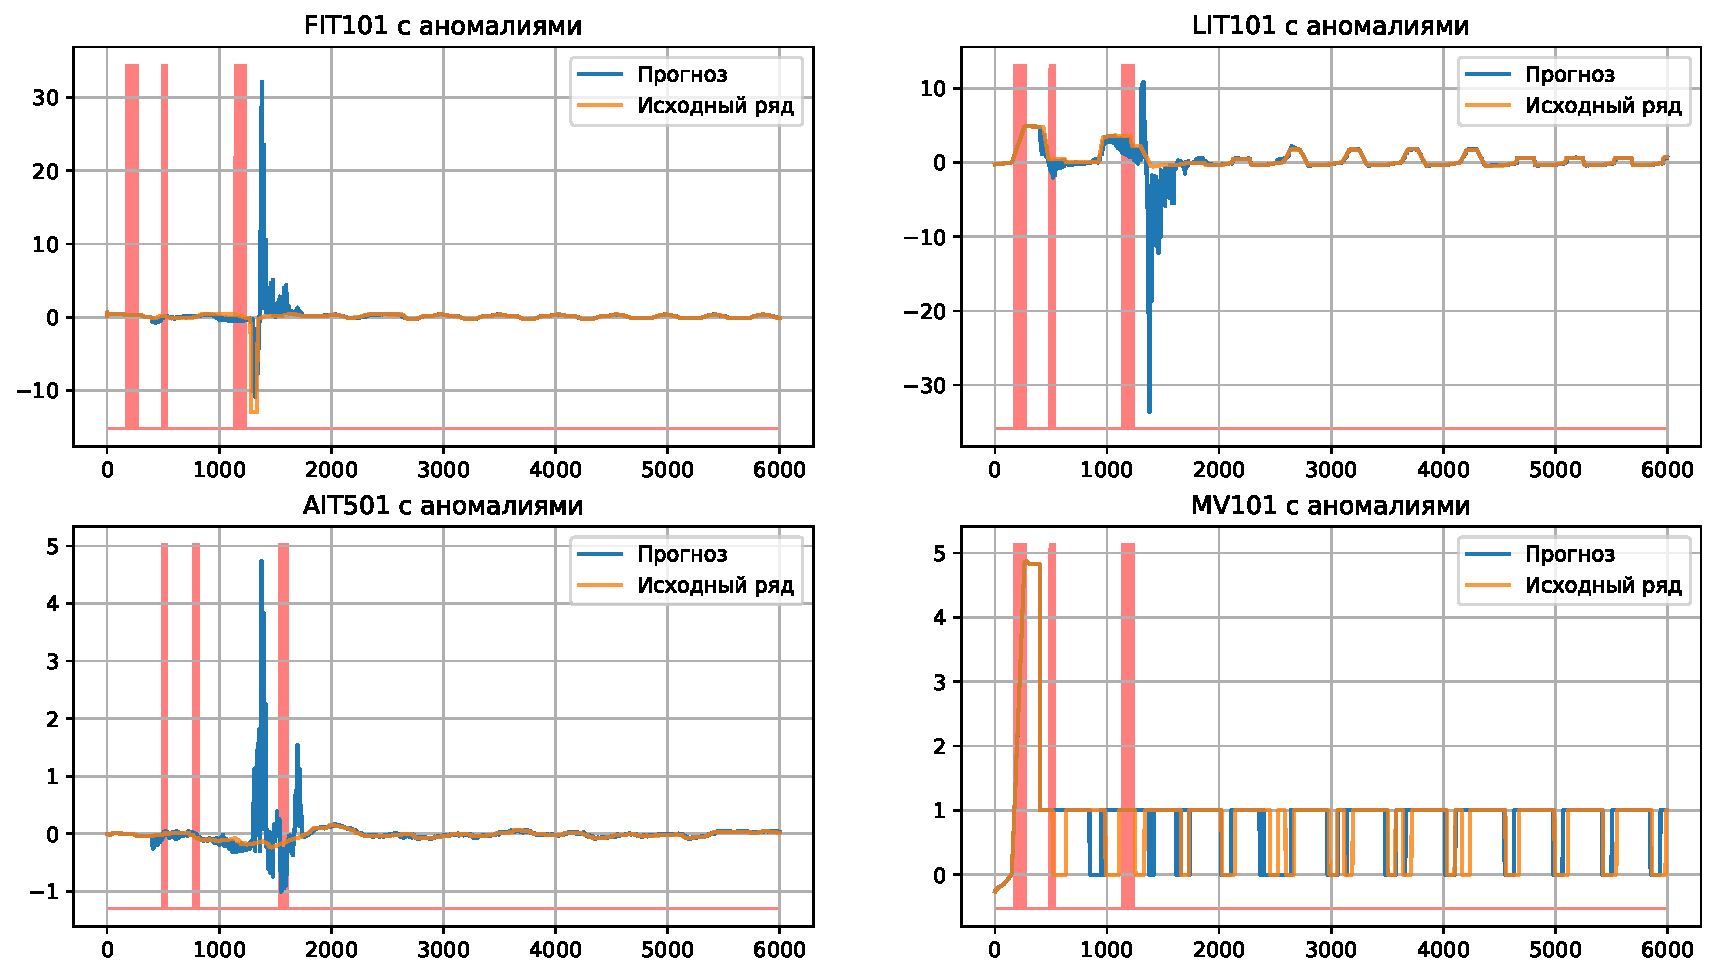
\includegraphics[width=0.9\textwidth]{Ano_pred_TCN.pdf}
\caption{Пример прогноза TCN для аномальных данных. Красным цветом отмечены аномальные зоны для данного ряда. Видно, что в аномальных зонах предсказанные значения существенно отличаются от типичных.}
\label{Ano_TCN}
\end{figure}

\begin{figure}[H]
\centering
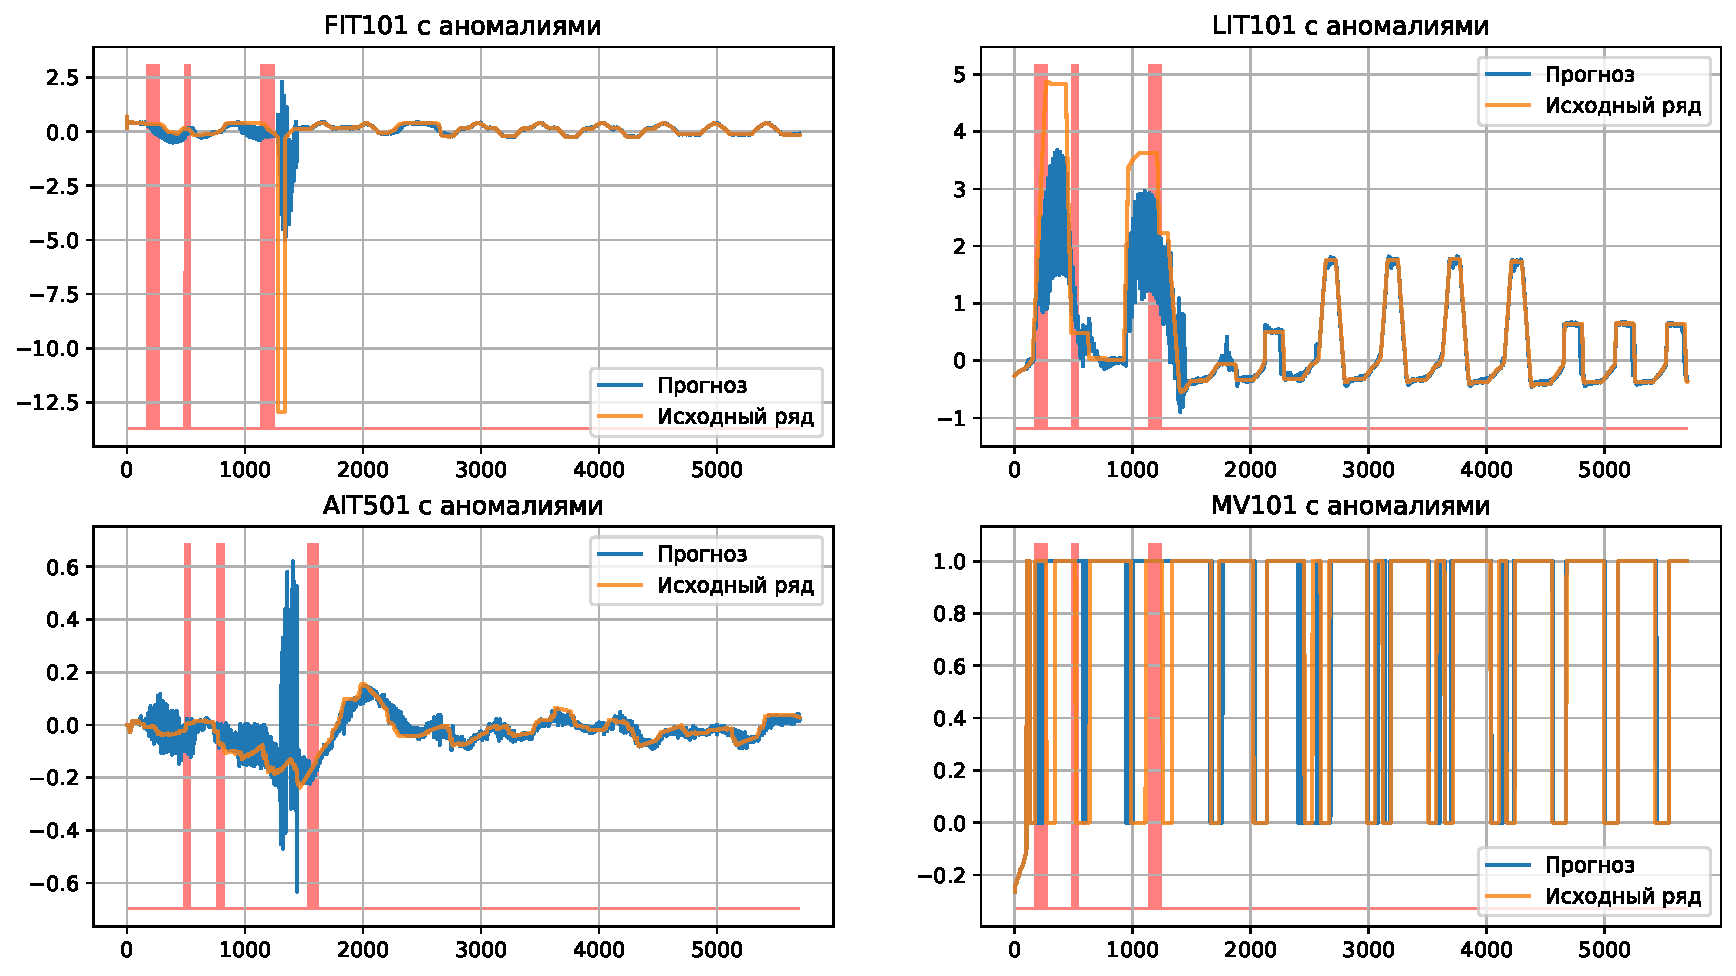
\includegraphics[width=0.9\textwidth]{Ano_pred_AF.pdf}
\caption{Пример прогноза Autoformer для аномальных данных.}
\label{Ano_AF}
\end{figure}

Для каждого ряда был подсчитан модуль разности $d$ предсказанных значений $y$ и исходных значений ряда $x$. Для момента времени $t$:

$d_t = |y_t - x_t|$

Дополнительно значения $d$ были преобразованы с помощью экспоненциального сглаживания: 

$s_1 = d_1,$

$s_t = \alpha d_t + (1 - \alpha)s_{t-1},  t > 1,  \alpha = 1 - \exp(\frac{\log(0.5)}{100})$

Значения $s$ для ряда 'FIT101' представлены на рис.\ref{FIT101_S}. 'Пики' значений s приходятся на аномальные зоны, при этом у модели TCN они более выраженные.

\begin{figure}[H]
\centering
\subcaptionbox{TCN}{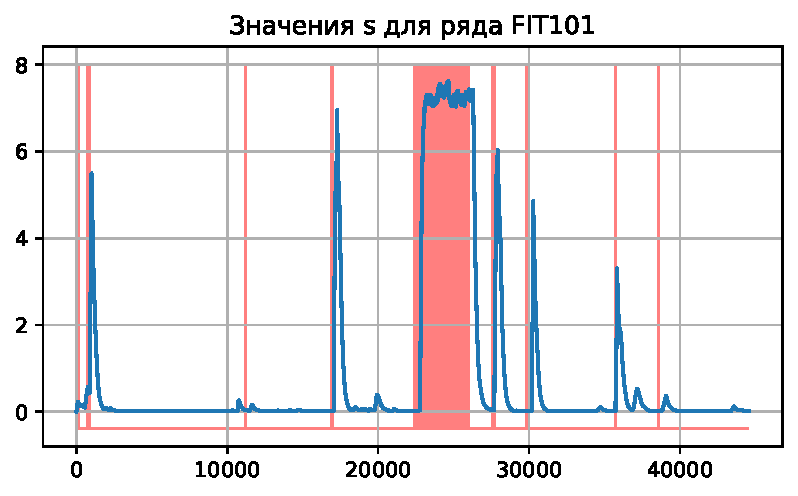
\includegraphics[width=0.5\textwidth]{FIT101_TCN.pdf}}%
\hfill
\subcaptionbox{Autoformer}{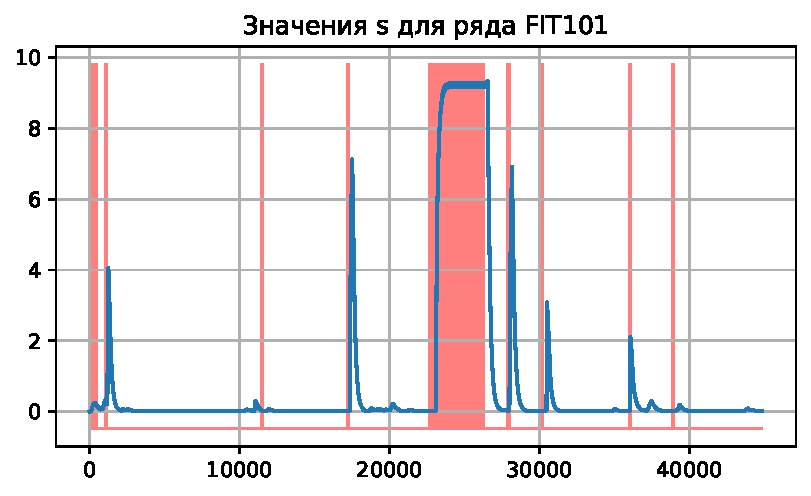
\includegraphics[width=0.5\textwidth]{FIT101_AF.pdf}}%
\caption{Значения разности s для ряда 'FIT101'. Красным цветом отмечены аномальные зоны.}
\label{FIT101_S}
\end{figure}

Детекция аномалий на всей аномальной выборке по порогу представлена на рис. \ref{FIT101_D}. Можно заметить, что графики обнаружения аномалий для моделей получились очень похожими - разная точность предсказаний всё равно позволила достаточно точно подобрать порог для обнаружения. Также видно, что все аномальные зоны из разметки менее протяжённые, чем зафиксированные - это связано с тем, что нестандартное поведение значений наблюдается не только во время самой атаки на систему, но и во время стабилизации после неё. Более того, некоторые атаки оказывают влияние на параметры процесса не сразу, а через небольшой промежуток времени, поэтому может наблюдаться задержка в обнаружении. По этой причине стандартные метрики, такие как точность, полнота и F1-мера, не будут в полной мере отражать качество обнаружения аномалий. При оценке качества обнаружения аномалий необходимо учитывать и сам факт обнаружения, поэтому для сравнения моделей были подсчитаны доли обнаруженных аномальных зон и средняя задержка обнаружения. Для определения факта обнаружения от каждой аномальной зоны из разметки и от зафиксированной аномальной зоны был оставлен только первый элемент. Результаты сравнения представлены в таблице.\ref{compar}. 

\begin{figure}[H]
\centering
\subcaptionbox{TCN}{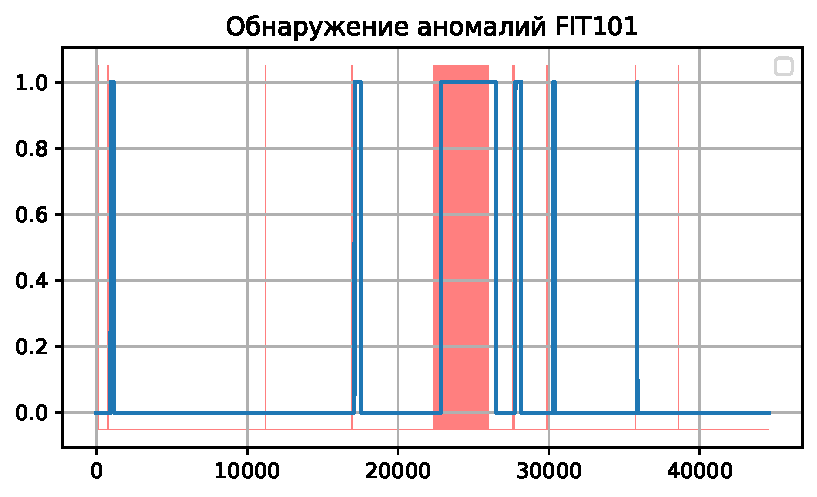
\includegraphics[width=0.5\textwidth]{FIT101_TCN_DETECTION.pdf}}%
\hfill
\subcaptionbox{Autoformer}{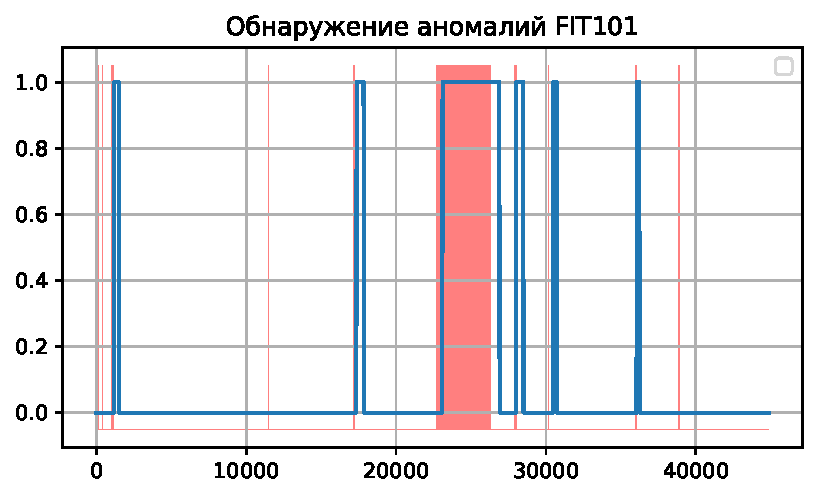
\includegraphics[width=0.5\textwidth]{FIT101_AF_DETECTION.pdf}}%
\caption{Обнаружение аномалий для ряда 'FIT101'. Красным цветом отмечены аномальные зоны. Значение 1 показывает, что в данный момент времени зафиксирована аномалия.}
\label{FIT101_D}
\end{figure}

Второй метод обнаружения аномалий на основе вероятностного подхода использовать не удалось: исследования показали, что значения стандартного отклонения при прогнозе аномального ряда существенно не отличаются от значений при прогнозе для данных без аномалий. А анализ среднего значения распределения эквивалентен первому методу. По этой причине дальнейшее исследование вероятностного подхода в данной работе не приводится. 

\begin{table}[h]
\centering
\begin{tabular}{|c|c|c|c|c|c|c|c|c|}
\hline
Модель & \begin{tabular}[c]{@{}c@{}}Точ-\\ ность,\\  \%\end{tabular} & \begin{tabular}[c]{@{}c@{}}Пол-\\ нота,\\  \%\end{tabular} & \begin{tabular}[c]{@{}c@{}}F1, \\ \%\end{tabular} & \begin{tabular}[c]{@{}c@{}}Точ-\\ ность \\ (с), \%\end{tabular} & \begin{tabular}[c]{@{}c@{}}Пол-\\ нота \\ (с), \%\end{tabular} & \begin{tabular}[c]{@{}c@{}}F1 \\ (с), \%\end{tabular} & \begin{tabular}[c]{@{}c@{}}Доля \\ обн-х\\ аномалий\end{tabular} & AD \\ \hline
TCN & 65.0 & 77.0 & 70.4 & 77.9 & 92.3 & 84.5 & 0.66 & 199.6 \\ \hline
Autoformer & 58.1 & 76.8 & 66.2 & 69.9 & 92.4 & 79.6 & 0.6 & 199.1 \\ \hline
TimesNet & 58.4 & 78.7 & 67.0 & 69.7 & 94.0 & 80.1 & 0.66 & 198.0 \\ \hline
\end{tabular}
\caption{Результаты сравнения моделей для ряда 'FIT101'. AD - средняя задержка обнаружения. Точность (с), полнота (с) и F1-мера (с) - метрики, подсчитанные для обнаруженных зон, сдвинутых на 400 шагов назад. При сдвиге значения метрик выше, так как наблюдается задержка обнаружения аномалий. }
\label{compar}
\end{table}
\subsubsection{Результаты экспериментов}
\begin{itemize}
\item Все рассмотренные в данном эксперименте модели способны точно предсказывать нормальные значения вещественнозначных рядов с выраженной периодичностью. Дискретные ряды также предсказываются достаточно хорошо - модели запоминают периоды, в которых значение остаётся постоянным, но нередко ошибаются в 'переходных' зонах изменения величины с одного значения на другое. Хорошо предсказывать вещественнозначный ряд без ярко выраженной периодичности не получилось, но модели TCN и Autoformer смогли выучить 'типичное' поведение значений этого ряда, что позволило использовать их прогноз для обнаружения аномалий и для такого ряда. 

\item Модель TCN, являясь наболее простой из рассматриваемых, смогла показать наилучшую точность прогноза нормальных данных. 

\item Рассмотренный метод обнаружения аномалий на основе разности значений прогноза и исходного ряда позволил фиксировать аномалии с достаточно высоким качеством. Требуемой точности обнаружения не удалось достичь только для дискретного ряда - выбор порога позволяет фиксировать либо слишком малое число настоящих аномалий, либо слишком большое число ложных аномалий. Метод обнаружения на основе вероятностного подхода не удалось использовать для обнаружения аномалий, не зафиксированных первым методом.

\item Несмотря на разную точность прогноза, пороги для обнаружения аномалий могут быть подобраны так, что качество обнаружения у разных моделей будет близким. Также метод на основе разности позволяет подбирать пороги и по нормальным данным, если отсутсвует выборка с аномалиями. 
\end{itemize}

\section{Анализ результатов}
В данной работе рассматривается выборка небольшого размера. Это приводит к тому, что данных может быть недостаточно для обучения рассматриваемых тяжёлых нейросетевых архитектур. Однако такого объёма данных достаточно для обучения рассматриваемой архитектуры TCN. На выборках существенно большего размера архитектуры Autoformer и TimesNet достигают лучших результатов, но при этом требуют значительно больше времени для обучения. Таким образом, TCN является хорошей архитектурой для выборок небольшого размера.

\section{Вывод}
В данной работе были рассмотрены архитектуры нейронных сетей для прогнозирования временных рядов и методы обнаружения аномалий на основе полученного прогноза. 

Был проведен эксперимент по исследованию и сравнению рекурретных и временных свёрточных сетей, в ходе которого было установлено, что временные свёрточные сети лучше справляются с задачей определения и запоминания долговременных связей в последовательностях и больше подходят для задачи прогнозирования временных рядов. 

Был проведён эксперимент по оценке качества прогноза и обнаружения аномалий моделями TCN, Autoformer и TimesNet, и были проанализированы два метода обнаружения аномалий: на основе разности значений и на основе вероятностного подхода. По результатам эксперимента можно сделать вывод, что рассмотренные модели и метод на основе разности значений хорошо подходят для решения поставленной задачи обнаружения аномалий.

В ходе сравнения моделей показано, что у TCN качество прогноза многомерного временного ряда выше, чем у Autoformer и TimesNet, созданных специально для этой задачи, - это открывает возможности для дальнейшего сравнения TCN с более сложными архитектурами и изучения качества TCN в других задачах, связанных с временными рядами.

\bibliographystyle{unsrtnat}
\bibliography{references}

\end{document}